\documentclass[11pt,a4paper]{article}
\usepackage[T1]{fontenc}
\usepackage[utf8]{inputenc}
\usepackage{lmodern,microtype,amsmath,amssymb,graphicx,booktabs,array,longtable,caption,geometry,titlesec,xcolor}
\usepackage[numbers,sort&compress]{natbib}
\usepackage[colorlinks=true,linkcolor=blue!50!black,citecolor=blue!50!black,urlcolor=blue!50!black]{hyperref}
\geometry{left=2.5cm,right=2.5cm,top=1.8cm,bottom=2.5cm}
\captionsetup{font=footnotesize,labelfont=bf,skip=3pt}
\titleformat{\section}{\normalfont\large\bfseries}{\thesection}{.6em}{}
\titleformat{\subsection}{\normalfont\normalsize\bfseries}{\thesubsection}{.6em}{}
\titlespacing*{\section}{0pt}{1.3ex plus .2ex minus .1ex}{.65ex}
\titlespacing*{\subsection}{0pt}{.9ex plus .1ex}{.4ex}
\setlength{\parindent}{1em}
\setlength{\parskip}{0pt}
\setlength{\textfloatsep}{7pt plus 1pt minus 1pt}
\setlength{\floatsep}{6pt plus 1pt minus 1pt}
\setlength{\intextsep}{6pt plus 1pt minus 1pt}
\setlength{\abovedisplayskip}{5pt plus 1pt minus 1pt}
\setlength{\belowdisplayskip}{5pt plus 1pt minus 1pt}
\renewcommand{\topfraction}{.95}
\renewcommand{\bottomfraction}{.95}
\renewcommand{\textfraction}{.05}
\renewcommand{\floatpagefraction}{.8}
\setcounter{topnumber}{3}
\setcounter{bottomnumber}{3}
\setcounter{totalnumber}{5}
\newcommand{\arcsinh}{\operatorname{asinh}}
\newcommand{\relu}{\operatorname{ReLU}}
\newcommand{\supp}[1]{Supplement~#1}
\graphicspath{{figures/}{figures/supplement/}}

\begin{document}
\begin{center}
{\Large\bfseries Benchmarking Comparative Single-Cell Analysis\\of CMV Status\par}
\vspace{3pt}
Sebastian Fay \quad Marie Schygulla \quad Gregor Habitzreither
\end{center}
\vspace{-6pt}

\section{Introduction}
Single-cell protein measurements describe many immune cells from each donor, but a clinical label such as cytomegalovirus (CMV) status applies to the donor. Only a small subset of cells may carry an associated phenotype, and cells from one donor are not independent biological replicates. CellCNN addresses this mismatch by jointly learning cell filters, pooling and donor prediction, allowing rare, informative responses to influence the representation~\cite{cellcnn}. We compare it with Citrus, which classifies donors using cluster frequencies~\cite{citrus}, and a single-cell SVM, which learns cell scores from donor labels and aggregates them for prediction.

The supplied cohort derives from Horowitz et al.~\cite{horowitz}, who link CMV exposure to NKG2C/CD57-expressing natural killer (NK) populations. We examine the cell landscape using dimensionality reduction and clustering, compare prediction on held-out donors, and assess model-associated subsets. A final experiment modifies CellCNN responses and pooling. Donor prediction and recovery of an informative population are evaluated separately.

\section{Methods}
\subsection{Dataset and preprocessing}
The mass-cytometry (CyTOF) data comprise 20 donors (9 CMV-positive, 11 negative) and 37 protein markers. Technical channels are excluded. After qualitatively comparing ArcSinh cofactors, we chose the default 5 (\supp{S1}). ArcSinh compresses large intensities and retains finite negative background values. We use $a=\arcsinh(x/5)$ and donor-balanced samples, with distinct analysis scopes: 40,000 \texttt{gated\_NK} cells for dimensionality reduction (2,000/donor), 20,000 \texttt{gated\_alive} PBMCs for clustering (1,000/donor), and \texttt{gated\_alive} for classification. The latter contains 3,438,750 events. The interpretation map contains 10,000 cells (500/donor), but selected-cell profiles use full test donors. Exploratory marker scaling uses the corresponding analysis sample. Classifier scaling is fitted only on training donors. Data checks and sampling details are in \supp{S1}.

\subsection{Dimensionality reduction}
PCA retains 29 components explaining 91.50\% of variance. These form the reference for t-SNE, UMAP and embedding-quality measurements. We sweep six t-SNE perplexities~\cite{tsne} and 64 UMAP settings~\cite{umap} on 5,000 cells. Trustworthiness $T(15)$~\cite{trust} selects the configuration. For UMAP, learning rate is first selected by mean $T$ across two fixed configurations, followed by neighbour count and minimum distance. Selected settings are fitted to all 40,000 cells. For direct comparison of every pair of final maps we use Procrustes disparity $M^2$, the residual after optimal translation, rotation/reflection and scaling~\cite{scipy}. Lower values mean closer aligned shapes. Trustworthiness penalises neighbours introduced by projection that were distant in the 29-PC space. It therefore measures a different property from agreement between two displayed maps. Additional neighbourhood and distance measures appear in \supp{S2}.

\subsection{Clustering and biological interpretation}
We cluster standardised 37-marker PBMC profiles, not two-dimensional projections~\cite{scipy,sklearn}. The 44 configurations cover centroid-based k-means, four hierarchical linkages including minimum-variance Ward, and Leiden communities on a weighted neighbour graph~\cite{leiden}. Davies--Bouldin (DB)~\cite{db} assesses one partition's compactness/separation; stability tests persistence after removing 20\% of initially sampled cells per donor and refitting scaling and clustering. Within each method/linkage, stability $\geq0.6$ establishes eligibility, then DB ranks configurations, avoiding an arbitrary weighted trade-off between geometry and reproducibility. Cluster-wise Jaccard tracks populations individually with equal cluster weights, unlike global measures such as ARI that can be dominated by large groups. Ten-repeat stability is the mean of cluster-wise median overlaps. Tiny clusters can appear stable whenever retained, so cluster size remains essential. Marker profiles are $(\text{cluster median}-\text{sample median})/\text{sample IQR}$ after ArcSinh (\supp{S2}).

\begin{figure}[tb]
\centering
\includegraphics[width=\linewidth]{v02/dimensionality_reduction.pdf}
\caption{The same 40,000 NK-gated cells coloured by donor CMV status. $T(15)$ measures neighbourhood preservation relative to 29 PCs. Procrustes disparity after alignment is 0.442 for PCA/t-SNE, 0.554 for PCA/UMAP and 0.368 for t-SNE/UMAP. Lower disparity indicates closer aligned shapes.}
\label{fig:dr}
\end{figure}

\subsection{Comparative single-cell classification}
The benchmark uses 30 shared donor splits: 14 training donors (7 per class), six test donors (2 positive, 4 negative), and three inner folds for model selection. Test donors never enter training fits. \textbf{CellCNN} uses 3--5 linear/ReLU filters, means of the top 1\% responses and a softmax output. Our PyTorch implementation retains the selected inner-fold network, trained on 9 or 10 donors, and averages five test-input probabilities. \textbf{Citrus} uses its original R implementation: Ward clusters, cluster-frequency features and L1-logistic regression. \textbf{SVM} uses a linear cell scorer trained with donor labels, and its donor score averages the highest 1\% of full-donor margins. Citrus and SVM are refitted on all 14 training donors. Our SVM aggregation and fixed CellCNN filter search are project adaptations. CellCNN and Citrus use a decision threshold of 0.5. The SVM threshold is selected on inner out-of-fold donor scores. Full implementation details are in \supp{S3}.

\subsection{Identification of model-associated subsets}
We select cells supporting the CMV-positive prediction. CellCNN selects cells exceeding half the training-reference maximum of any active filter weighted toward CMV-positive donors. SVM selects cells among the donor's highest-scoring 1\% whose scores exceed its inner-trained decision threshold. Citrus selects cells assigned to a positively weighted training cluster, transferring memberships from the nearest original training cell. Each cell counts once per split. Its displayed selection frequency is the proportion of its donor's test appearances in which it is selected, including appearances with empty selections. Marker profiles average selected cells within nonempty test appearances, then appearances within donors and donors equally. Selection rules and Figure~\ref{fig:subsets} interpretation are detailed in \supp{S3.2--S3.3}.

\section{Results}
\subsection{Dimensionality reduction}
The two-dimensional PCA map retains only 20.29\% of variance. In the sweep, t-SNE trustworthiness rises from 0.8931 at perplexity 5 to 0.9235 at 30, peaks at 0.9271 for 70, and varies little across 30--100. Low perplexity emphasises very local arrangements, whereas higher values change the scale of visible neighbourhoods. For UMAP, smaller minimum distance packs points more tightly and neighbour count changes local connectivity. Learning rate also affects the result (\supp{S2}). The UMAP learning-rate selection score drops from 0.8781 at rate 0.1 to 0.8589 at rate 5. The selected setting is 5 neighbours, minimum distance 0 and learning rate 0.1.

On the final 40,000-cell maps, t-SNE has the highest $T$ (0.9608), ahead of UMAP (0.8838) and PCA (0.7258). PCA preserves pairwise distances better in the 2,000-cell distance sample ($r=0.6204$, versus 0.4799 and 0.4317). Thus local and global criteria favour different methods. t-SNE and UMAP are the most similar pair under Procrustes ($M^2=0.3683$, Fig.~\ref{fig:dr}). Donor CMV classes remain substantially intermixed. A visible island alone is neither a cell-type annotation nor a classification result.

\begin{figure}[htb]
\centering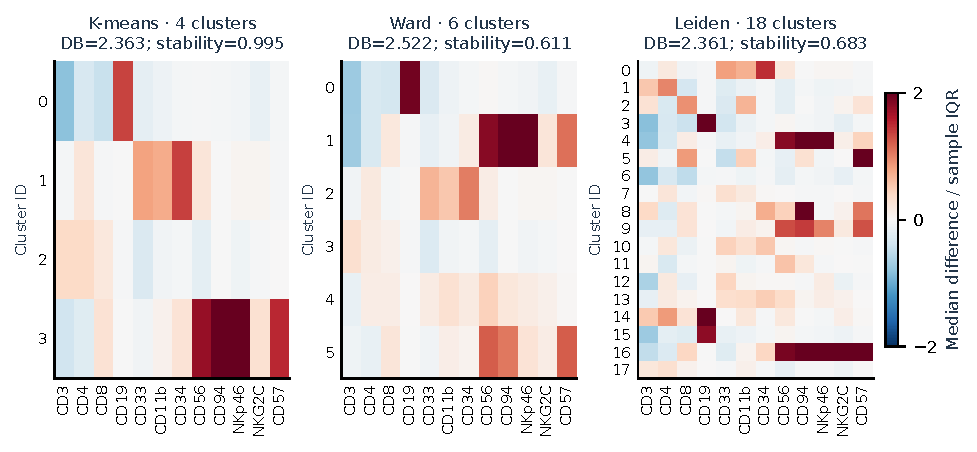
\includegraphics[width=\linewidth]{clustering.pdf}
\caption{Marker evidence for the selected k-means, Ward and Leiden solutions on 20,000 live PBMCs. Twelve markers share one relative-IQR scale with colours clipped at $\pm2$. Cluster IDs are local to each method. DB is evaluated in 37D. Stability comes from the original ten cell-subsampling repeats. Full profiles appear in \supp{S2}.}
\label{fig:clusters}
\end{figure}

\subsection{Clustering and biological interpretation}
K-means selects four broad groups with mean stability 0.995. Ward yields six groups (0.611), and Leiden 18 (0.683). The DB scores of k-means and Leiden are nearly equal (Fig.~\ref{fig:clusters}). K-means separates CD19-enriched and NKp46/CD94-enriched groups, while Ward separates CD19-enriched and CD56/CD94/NKp46-enriched groups. Compared with the coarse k-means solution, Leiden resolves a strongly NKG2C/CD57-enriched group of 281 cells. These descriptions concern relative marker medians, not validated cell-type labels or proof of single-cell co-expression.

DB weights clusters equally, whereas a global mean silhouette weights them by cell count. This avoids automatically downweighting rare populations, but also gives small artefactual groups influence: single linkage separates 19,999 cells from one event despite DB $=0.264$ and stability $=1$. Thus DB and stability require interpretation alongside cluster sizes and marker profiles. Three of six Ward clusters and four of 18 Leiden clusters have stability below 0.6 even though their averages pass. K-means is the strongest reproducible coarse description here. Ward and Leiden offer subdivisions requiring validation. Cell-removal stability within this cohort does not establish replication in new donors or a biologically superior partition without reference annotations.

\subsection{Classification benchmark}
CellCNN and SVM both achieve median test AUC 0.875, compared with 0.625 for Citrus (Fig.~\ref{fig:benchmark}). CellCNN exceeds SVM in 12 splits, ties in 12 and falls below it in six. Its mean paired AUC advantage is only 0.0167. Against Citrus, the corresponding counts are 22/6/2. Median balanced accuracy is 0.625 for CellCNN/SVM and 0.500 for Citrus, showing that good rankings do not automatically produce strong thresholded decisions. Each test set supplies only eight positive--negative donor pairs, making AUC sensitive to individual rankings. Repeated splits therefore describe variation within this cohort. Complete metric distributions are in \supp{S5}.

\begin{figure}[tb]
\centering
\includegraphics[width=\linewidth]{v02/classification.pdf}
\caption{Performance on 30 shared splits of 20 donors. A shows test AUC and B shows paired AUC differences on identical splits. Boxes span Q1--Q3 with median lines and whiskers to the most extreme values within 1.5 IQR of the box. Dots are splits. Counts denote better/equal/worse performance of the first method. Overlapping splits describe variation within this cohort, not confidence intervals.}
\label{fig:benchmark}
\end{figure}

\subsection{Model-associated cell subsets}
The common test-cell analysis reveals different selection patterns (Fig.~\ref{fig:subsets}). CellCNN, SVM and Citrus select 863, 93 and 1,583 map cells at least once, but only 84, 9 and 11 in at least half of their donor's test appearances. CellCNN has a consistent core within a broader, less stable selection, whereas Citrus marks many cells intermittently. Fifteen CellCNN reference cells are selected in every test appearance, compared with none for SVM or Citrus. Each cell counts only once per split, so recurrence reflects reproducibility of its selection rather than the number of filters or nested clusters selecting it. CellCNN/SVM profiles show stronger NKG2C enrichment (mean reference z-scores 2.862/3.004) than Citrus (0.972), alongside NK-associated markers. This is compatible with the CMV-related phenotype described by Horowitz et al.~\cite{horowitz}, but the pooled profiles can mix populations. Tracking the same cells permits comparison without aligning individual filters or clusters between splits. Different selection rules prevent interpreting cell counts alone as biological superiority.

\begin{figure}[htb]
\centering
\includegraphics[width=\linewidth]{v02/subsets.pdf}
\caption{A--C show the same 10,000 \texttt{gated\_alive} reference cells on t-SNE (perplexity 30). Colour is selections divided by the donor's 4--16 outer test appearances across 30 splits. Grey means never selected. Panel counts indicate selection at least once and in at least half of test appearances. D shows full-test-donor marker profiles on a common z-scale, averaging selected cells within nonempty test appearances, then appearances within donors and all 20 donors equally. Empty selections remain in frequency denominators but have no marker profile. Selection rules differ by method.}
\label{fig:subsets}
\end{figure}

\subsection{Exploratory extension: modified CellCNN}
\label{sec:bonus}
We use $r_f(z)=\relu(b_f+w_f^Tz+\sum_j q_{fj}z_j^2)$ for standardised marker vector $z$ and filter $f$. This adds marker-wise curvature without cross-marker products $z_jz_\ell$. Starting at $q=0$ recovers the linear response. L2 penalises added curvature, so training gains must justify its penalty. We compare hard top-1\% and learnable soft-fraction pooling with a diagonal Mahalanobis/ReLU prototype model. Its geometry penalty instead pulls axis weights toward one (isotropy). With only 20 donors, including identical twins, using 37 diagonal weights rather than 703 full symmetric entries per filter limits cohort-specific fitting (\supp{S4}).

Network AUC evaluates full-representation donor predictions. Frequency AUC tests whether one high-response population's frequency separates CMV-positive and negative test donors. Per model/split, the filter with the largest positive output contrast and its inner-training half-maximum threshold define the population. Its frequency on fixed test-donor samples supplies the ROC-AUC score. Network/frequency comparisons use 100/98 jointly evaluable splits, respectively.

Both quadratic variants improve mean network AUC by 0.1050 without a comparable frequency-AUC gain (table below; paired differences in \supp{S5}). Better donor prediction therefore does not establish better recovery of a single phenotype-associated rare population. Soft pooling adds no clear advantage. The prototype performs worse in both analyses, but different initialisation and regularisation prevent attributing this purely to Mahalanobis geometry.

\begin{center}\small
\begin{tabular}{@{}lrr@{}}\toprule
Model & Mean network AUC & Mean frequency AUC\\\midrule
CellCNN baseline & 0.8075 & 0.8559\\
Quadratic Top-1\% & 0.9125 & 0.8610\\
Quadratic Soft-$\alpha$ & 0.9125 & 0.8559\\
Mahalanobis/ReLU Soft-$\alpha$ & 0.7375 & 0.7245\\\bottomrule
\end{tabular}
\end{center}

\section{Discussion and conclusion}
Embedding quality describes geometry, clustering stability reproducibility within sampled cells, and classification held-out donor prediction. Network prediction, CMV association of a selected population's frequency and reproducibility of cell selection are separate targets. None alone validates a biological cell type. The 20 donors include four identifiable pairs of identical twins; overlapping splits and heuristic subset thresholds further limit generalisation. CellCNN and SVM give similar rankings but different selections. Citrus is weaker here.

The benchmark compares complete implementations: CellCNN retains an inner-fold model while baselines refit on all training donors, and donor input sizes differ. Differences cannot therefore be attributed solely to model family. Equal cell sampling cannot replace independent donors. Future evaluation should keep twin pairs together and test subset-threshold sensitivity against reference annotations. Quadratic filters improve donor-level network prediction in this cohort, with little or no gain in the selected rare-population signal. These exploratory findings require independent donors and biological assessment of selected cells.

\begingroup
\footnotesize
\raggedright
\setlength{\bibsep}{1.5pt}
\begin{thebibliography}{10}
\bibitem{cellcnn} E.~Arvaniti and M.~Claassen. Sensitive detection of rare disease-associated cell subsets via representation learning. \emph{Nat. Commun.} 8:14825, 2017. \href{https://doi.org/10.1038/ncomms14825}{doi:10.1038/ncomms14825}.
\bibitem{horowitz} A.~Horowitz et al. Genetic and environmental determinants of human NK cell diversity revealed by mass cytometry. \emph{Sci. Transl. Med.} 5:208ra145, 2013. \href{https://doi.org/10.1126/scitranslmed.3006702}{doi:10.1126/scitranslmed.3006702}.
\bibitem{citrus} R.~V.~Bruggner et al. Automated identification of stratifying signatures in cellular subpopulations. \emph{PNAS} 111:E2770--E2777, 2014. \href{https://doi.org/10.1073/pnas.1408792111}{doi:10.1073/pnas.1408792111}.
\bibitem{tsne} L.~van der Maaten and G.~Hinton. Visualizing data using t-SNE. \emph{JMLR} 9:2579--2605, 2008. \href{https://www.jmlr.org/papers/v9/vandermaaten08a.html}{jmlr.org/papers/v9/vandermaaten08a.html}.
\bibitem{umap} L.~McInnes, J.~Healy and J.~Melville. UMAP: Uniform manifold approximation and projection for dimension reduction. \emph{arXiv:1802.03426}, 2018. \href{https://doi.org/10.48550/arXiv.1802.03426}{doi:10.48550/arXiv.1802.03426}.
\bibitem{trust} J.~Venna and S.~Kaski. Neighborhood preservation in nonlinear projection methods: an experimental study. \emph{ICANN}, pp.~485--491, 2001. \href{https://doi.org/10.1007/3-540-44668-0_68}{doi:10.1007/3-540-44668-0\_68}.
\bibitem{db} D.~L.~Davies and D.~W.~Bouldin. A cluster separation measure. \emph{IEEE TPAMI} PAMI-1:224--227, 1979. \href{https://doi.org/10.1109/TPAMI.1979.4766909}{doi:10.1109/TPAMI.1979.4766909}.
\bibitem{leiden} V.~A.~Traag, L.~Waltman and N.~J.~van Eck. From Louvain to Leiden: guaranteeing well-connected communities. \emph{Sci. Rep.} 9:5233, 2019. \href{https://doi.org/10.1038/s41598-019-41695-z}{doi:10.1038/s41598-019-41695-z}.
\bibitem{scipy} P.~Virtanen et al. SciPy 1.0: fundamental algorithms for scientific computing in Python. \emph{Nat. Methods} 17:261--272, 2020. \href{https://doi.org/10.1038/s41592-019-0686-2}{doi:10.1038/s41592-019-0686-2}.
\bibitem{sklearn} F.~Pedregosa et al. Scikit-learn: machine learning in Python. \emph{JMLR} 12:2825--2830, 2011. \href{https://www.jmlr.org/papers/v12/pedregosa11a.html}{jmlr.org/papers/v12/pedregosa11a.html}.
\end{thebibliography}
\endgroup


\end{document}
